\documentclass[conference]{IEEEtran}
\usepackage{blindtext, graphicx, hyperref, amsfonts, listings, bm}

\hyphenation{op-tical net-works semi-conduc-tor}
\begin{document}
\title{Product Recommendation by Rating-based Collaborative Filtering using Apache Spark}

\author{\IEEEauthorblockN{Songxiao Zhang}
\IEEEauthorblockA{Courant Institute of Mathematical\\
Sciences, New York University\\
sz1451@nyu.edu}
\and
\IEEEauthorblockN{Alan Yang}
\IEEEauthorblockA{Courant Institute of Mathematical\\
Sciences, New York University\\
asy233@nyu.edu}
\and
\IEEEauthorblockN{Suzanne McIntosh}
\IEEEauthorblockA{Courant Institute of Mathematical\\
Sciences, New York University\\
sm4971@nyu.edu}}

\maketitle

\begin{abstract}

What determines a good recommendation system?  In the modern society in which electronic commerce or E-commerce is becoming more and more popular and relevant, this becomes an interesting and potentially profitable question.  The main purpose of this project, is for us to explore whether or not we can create a solid recommendation system based on users reviewing certain products and giving these products a high rating.  To accomplish this goal we will be using collaborative filtering, which is a technique commonly used for recommendation systems.

There are two approaches to collaborative filtering (CF), namely memory-based CF and model-based CF \cite{Breese}. Memory-based CF systems utilizes an original and entire user-item rating matrix to generate predictions \cite{Resnick}. Model-based CF methods on the other hand, recommend items by first developing a descriptive model of user ratings based on an user-item matrix via different machine learning approaches such as Bayesian network and clustering. This generated model is then used for future prediction about the user's preferences \cite{Breese}. In this paper, we will be mainly looking into the model-based collaborative filtering approach and evaluating if the approach works well for our problem. 

\end{abstract}

\begin{IEEEkeywords}
collaborative filtering, memory-based CF, model-based CF, recommendation system. 
\end{IEEEkeywords}


\section{Introduction}

When consumers shop and browse on big E-commerce sites such as Amazon, they are prompted with other products that they may be interested in.  These products are recommended based on either the consumers search query, or on the consumers previously purchased products.  Amazon even has recommendation systems based on the idea of “Frequently Bought Together” and “Customers Who Bought This Item Also Bought” for whatever product the consumer is currently looking at.  
But what if we want to create a recommendation system that is based on a consumer reviewing a product and rating that product highly.  To be clearer we will consider a specific product “A” as a starting point.  A consumer Bill has reviewed and rated product “A” with five stars.  The next step will be finding all the other users who have given product “A” five stars.  Then all of the products in which these other users have rated five stars will be returned as the recommendation to consumer Bill for review product “A” highly.

This ideology is based on a technique called collaborative filtering.  Collaborative filtering is a technique that is highly used for recommendation systems.  As mentioned in the abstract, there are two approaches towards collaborative filtering: memory-based collaborative filtering and model-based collaborative \cite{Breese}.  Memory-based CF systems utilize an original, entire user-item rating matrix to generate predictions \cite{Resnick}, while model-based CF methods recommend items by first developing a descriptive model of user ratings based on a user-item matrix via different machine learning approaches such as Bayesian network and clustering. The generated model is then used for future prediction about user preferences \cite{Breese}.  In our specific analysis, we will be using Spark's MLlib library which supports collaborative filtering, namely the model-based algorithm called Alternating Least Squares (ALS).  The ALS model-based collaborative filtering technique learns a small set of latent factors which describes users and products in the data.  These latent factors can then be used to predict missing entries and recommend new products to users.

For this paper, we will only consider review data from Amazon.com and Yelp.com.  The data will be collected in bulk and will be preprocessed and used accordingly.  We will process the data so that for each review, we will have the reviewer (or user) ID, the product ID, and the rating for the product.

\section{Motivation}

Apache Spark is a new open source cluster computing framework. Spark is fast and a good general engine for large-scale data processing. Spark is said to run programs up to 100x faster than Hadoop MapReduce in memory, or 10x faster on disk \cite{ApacheSpark}. We want to explore how production recommendation can be done by collaborative filtering in rating based e-commerce systems in Spark. We want to investigate the speed and performance and see if it can be integrated to a real-time big data system. 

As one of libraries of Spark, MLlib is a scalable machine learning engine that consists of common learning algorithms and utilities, including classification, regression, clustering, collaborative filtering, dimensionality reduction, as well as lower-level optimization primitives and higher-level pipeline APIs. In MLlib, collaborative filtering is implemented by alternating least squares (ALS), which has been implemented in many machine learning libraries and widely studied and used in both academia and industry. We will see if ALS is the best candidate for product recommendation scenario. 

\section{Related Work}

Collaborative Filtering is based on the idea that after analyzing a large amount of information on user preferences, we should be able to predict what the user will like based on similar preferences with other users.

According to \cite{ClusteringItems}, collaborative filtering is most useful in certain situations in which the nearest neighbor model is used for research or commercial systems for generating predictions.  The nearest neighbor model works in three simple phases.  

\begin{enumerate}
  \item The first phase is collecting the appropriate data. This means that the users of whatever system must be able to rate
        items that they have previously experienced. 
  \item The second phase is that the collaborative filtering system will match the user to other participants of the system who
        have similar rating patterns.  This means that the user will share similar interests, opinions, or products as these 
        other participants based on what the collaborative filtering system is used for.  The participants who are closest 
        matched to the original user becomes known as neighbors to the original user, while collectively, all the neighbors 
        form a neighborhood.
  \item Finally, the last step of the model is that the items in which the neighbors have rated highly and the original user has
        never experienced is recommended to the original user.  The items are ranked based on closeness of the neighbor and the 
        consistency of opinion in the neighborhood.
\end{enumerate}

For clarity, if a person “Bob” has the same opinion on an issue as a different person “Alice”, then it is more likely for Bob to share the same opinion on another issue with Alice than with a random different person.  Therefore the issues in which Alice prefers or finds most interesting are the items in which are recommended to Bob.  The example is depicted in Figure 1 below.

\begin{figure}[h]
\centering
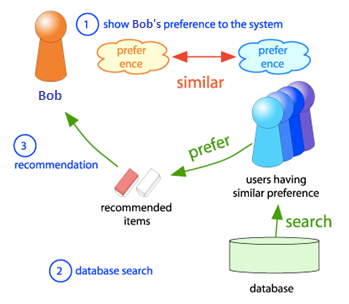
\includegraphics[width=0.5\textwidth]{image/cf_example_flow}
\caption{Example Flow of Collaborative Filtering}
\end{figure}

However, according to \cite{ClusteringItems}, there are some problem that arise with automated collaborative filtering that usually occurs with larger number of items in the prediction domain. These problems are very predictable:

\begin{enumerate}
  \item The first problem is that because users can only buy so many products or listen to so many songs or watch so many
        movies, the density of user ratings on the items available decreases with a larger item set.  Therefore, it becomes 
        less likely that many neighbors will have experienced and share a liking for a specific item as the user.
  \item The second problem is that even though there is a decreased density, the number of items to be considered between 
        each user and their neighbors increases which increases the amount of time necessary to compute the correlations in 
        the neighborhood.
  \item And finally and most importantly as the number of items increases, the items that a user likes becomes more different
        and diverse.  Therefore, it becomes less likely for there to be a correlation between the user’s opinions on a single
        item with all other items available.
\end{enumerate}

These problems make collaborative filtering hard to scale with larger data sets with more items.  These are definitely problems that we are vulnerable to for our project as we do deal with diverse and large item data sets with our Amazon and Yelp data.  O’Connor and Herlocker \cite{ClusteringItems} suggests that a solution is to partition the items based on user rating data.  Partitioning the items will result in fewer items, less ratings, and less users.  The hope is that by clustering together similar items, the prediction accuracy of the collaborative filtering will increase as there may be less noise.  However, although there is potential in certain partitioning algorithms such as kMetis graph partitioning algorithm, the results were that all of the partitioning algorithms resulted in a lower accuracy rate than the un-partitioned collaborative filtering results.  Therefore, our project will not be dealing with partitioning our data into clusters. 

\section{Design}

\subsection{Data Processing}

The review data we will be using for our analysis are from Yelp and Amazon.  The Yelp data was collected from the Yelp Data Set Challenge and Dr. Julian McAuley provided us with the Amazon review data.  The data was originally in JSON format.  Because the data collected are not in the proper structure in which we require, some data processing is required using Pig, Hive and Python.  Hive allows us to create data tables and remove columns in which we consider to be unnecessary.

Firstly, we created tables for each data set using Hive with only the specific columns necessary for our analysis. These  attribute columns are: User ID, Review ID, Rating, Date, and Product ID. The data must then be loaded, filtered, and processed accordingly with Pig so that we have a format which is easy to be used for our data analysis.

\begin{figure}[h]
\centering
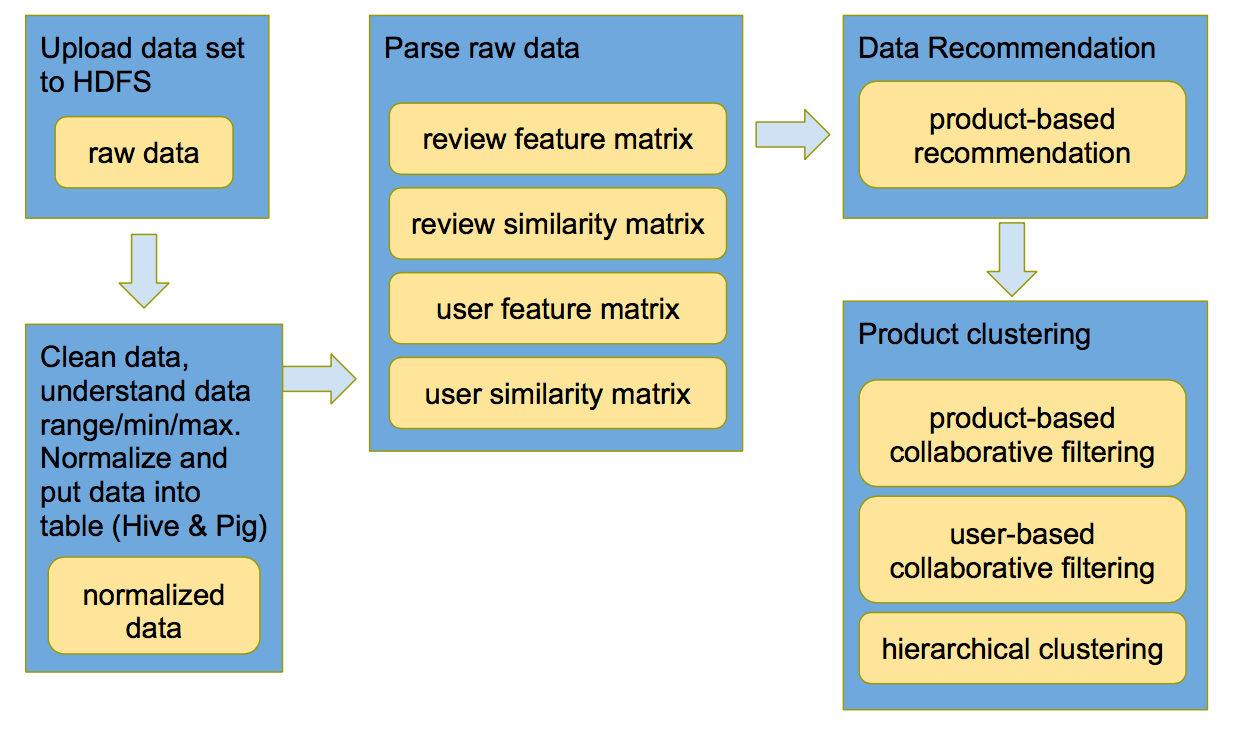
\includegraphics[width=0.5\textwidth]{image/design_diagram}
\caption{Design Diagram on Data Processing to Analysis}
\end{figure}

\subsection{Data Analysis Using Collaborative Filtering}

We used the MLlib library in Spark to run collaborative filtering. Spark MLlib implements a model-based collaborative filtering algorithm called Alternating Least Squares (ALS). ALS models the rating matrix (R) as the multiplication of low-rank user (U) and product (V) factors.  

% http://www.quuxlabs.com/blog/2010/09/matrix-factorization-a-simple-tutorial-and-implementation-in-python/

Let $\boldsymbol{R}$ of size $|U| \times |V|$ be the matrix that contains all the ratings that the users have assigned to the products or businesses. Also, we assume that we would like to discover $K$ latent features. Our task, then, is to find two metrics matrices $\boldsymbol{P}$ (a $|U| \times K$ matrix) and $\boldsymbol{Q}$ (a $|V| \times K$ matrix) such that their product approximates $\boldsymbol{R}$

$$ \boldsymbol{R \approx P \times Q^T = \hat{R}} $$

In this way, each row of $\boldsymbol{P}$ would represent the strength of the associations between a user and the features. Similarly, each row of $\boldsymbol{Q}$ would represent the strength of the associations between an item and the features. To get the prediction of a rating of an item $d_j$ by $u_i$, we can calculate the dot product of the two vectors corresponding to $u_i$ and $d_j$

$$ \hat{r}_{ij} = p^T_i q_j = \sum_{k=1}^{k}p_{ik} q_{kj} $$

Now, we have to find a way to obtain $\boldsymbol{P}$ and $\boldsymbol{Q}$. One way to approach this problem is the first intialize the two matrices with some values, calculate how `different’ their product is to $\boldsymbol{M}$, and then try to minimize this difference iteratively. Such a method is called gradient descent, aiming at finding a local minimum of the difference.

The difference here, usually called the error between the estimated rating and the real rating, can be calculated by the following equation for each user-item pair

$$ e^2_{ij} = (r_{ij} - \hat{r}_{ij})^2 = (r_{ij} - \sum_{k=1}^{K}p_{ik} q_{kj})^2 $$

ALS learns these factors by minimizing the reconstruction error of the observed ratings. The unknown ratings can subsequently be computed by multiplying these factors. In this way, companies can recommend products based on the predicted ratings and increase sales and customer satisfaction.


\begin{figure}[h]
\centering
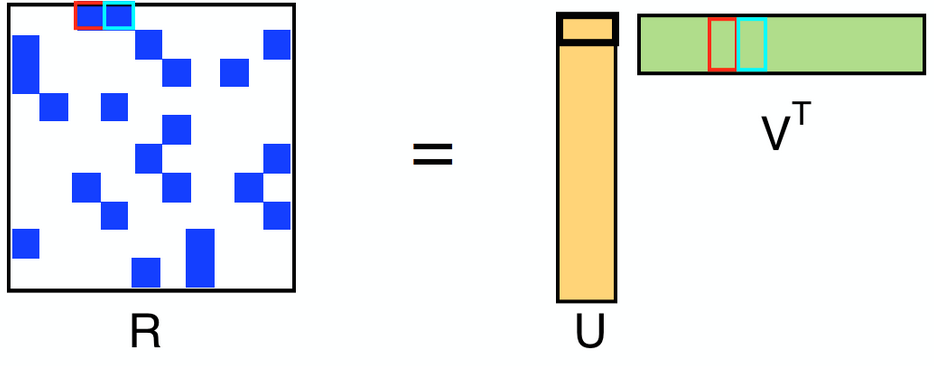
\includegraphics[width=0.4\textwidth]{image/als-illustration.png}
\caption{An illustration of ALS}
\end{figure}


Based on low-rank matrix factorization, we iterate through

$$U[i] = \min_{w \in \mathbb{R}^d} \sum_{j \in Nbrs(i))} (r_{ij} - w^TV^T[j])^2 + \lambda \left \| w \right \|^2_2$$


\subsection{ALS Implementation}

We will use MLlib’s ALS to train a MatrixFactorizationModel, which takes a RDD[(user, product, rating)] object as input. ALS has training parameters such as rank for matrix factors and regularization constants. To determine a good combination of the training parameters, we randomly split the data into three non-overlapping subsets, named training, test, and validation, based on the last digit of the timestamp, and cache them.  The distribution of or data for these three subsets are: 60 percent for training and 20 percent each of test and validation.  We will train multiple models based on the training set, select the best model on the validation set based on RMSE (Root Mean Squared Error), and finally evaluate the best model on the test set. We then take an input file with a specific user's ratings to the training set to make recommendations for that user. We hold the training, validation, and test sets in memory by calling cache because we need to visit them multiple times.

ALS is an iterative algorithm. In each iteration, the algorithm alternatively fixes one factor matrix and solves for the other, and this process continues until it converges. MLlib features a blocked implementation of the ALS algorithm that leverages Spark’s efficient support for distributed, iterative computation. It uses native LAPACK to achieve high performance and scales to billions of ratings on commodity clusters. 

MLlib's ALS algorithm has the following parameters \cite{ApacheSpark}:

\begin{itemize}
    \item numBlocks: the number of blocks used to parallelize computation (set to -1 to auto-configure).
    \item rank: the number of latent factors in the model.
    \item iterations: the number of iterations to run.
    \item lambda: the regularization parameter in ALS.
    \item implicitPrefs: specifies whether to use the explicit feedback ALS variant or one adapted for implicit feedback data.
    \item alpha: a parameter applicable to the implicit feedback variant of ALS that governs the baseline confidence in preference observations.
\end{itemize}

The review data collected uses unique identifiers (UID) as ids for but the reviewer/user and product.  These UIDs are generally in a numeric or alpha-numeric string format that is associated weith a single entity within a given system.  For example, a sample business id (product id from our Yelp review data) is u’JVmC54M6XBrjCBim71ELtw’ and a sample user id is u’A24m0MqrLlDXvZR9b69yOA’. 
The problem with MLlib's ALS algorithm in conjunction to our data, is that it's training function asks for Java int variables as its mapped training data, and so our alpha-numeric ids does not work without some data manipulation.  To solve this problem, hash functions were used to get an integer type in python, but the hashed value is too large and so is considered a long variable in Scala and Java which does not work for MLlib's specific parameter format.  This is because the implementation of MLlib is in Scala which uses Java underneath and both languages are strongly typed. When using Python, which is weakly typed, to run MLlib, a ClassCastException is thrown as the long variable type cannot be cast as an int variable type. Because Python has a wider integer range than Java, a larger type int was used with Python which is out of range of Java's int.

The solution to this problem is to use only a number of the last digits (should really be at least 8 digits for amazon data and 6 digits for yelp data). 

of the hashed values which is an integer within the range of a Java int type.
and handle hash collisions when we found the size of the list of all ids is bigger than the size of the set of all ids. 

The training, test, and validation subsets will then be used to find the best model and optimal parameters to train our data set, before applying the parameters into a specific user's ratings.


\section{results}

Sample model-based Collaborative Filtering results 

RMSE (validation) = 3.772036 for the model trained with rank = 16, lambda = 10.0, and numIter = 20.

RMSE (validation) = 3.775062 for the model trained with rank = 16, lambda = 10.0, and numIter = 30.

The best model was trained with rank = 16 and lambda = 0.1, and numIter = 20, and its RMSE on the test set is 1.486116.

The best model improves the baseline by -10.12$\%$.


\begin{lstlisting}
\end{lstlisting}


\section{future work}

We will add more data sources (e.g., "customers also bought") to cross-validate our results and give a accuracy rating. We will investigate into more specific, latest and trending topics for product recommendation such as what is the most prevailing Computer Graphics (CG) gears for Virtual Reality (VR) lovers. 

\section{Conclusion}

ALS is a Machine Learning algorithms generally use many iterations. Using MLlib to do collaborative filtering based recommendations is efficient as Spark is good at doing iterative jobs, comparing to Mahout. Spark does not write to disk on every iteration like Hadoop does which makes Hadoop much slower. This advantage makes MLlib scalable running machine learning algorithms. 

We found when developing applications using a language (Python in our case) rather than the language implementing the platform (Scala for Spark), we may encounter some incomptibility issue we mentioned in implementation section: Python int is bigger than Scala (Java) int so Java takes it as long, which does not work in ALS library as long is not casted to int automatically. So extra overhead and care need to be put on developing applications not using the language that the platform is implemented. 

\section*{Acknowledgment}

We would like to thank Professor Suzanne McIntosh advising and supervising us along this project. We'd also like to thank Dr. Julian McAuley from UCSD, Yelp Dataset Challenge board \cite{YelpDataset} and BestBuy API team who gave us dataset so we can conduct this research. Dr. Julian crawled Amazon review data before Amazon.com prevented us from web crawling. BestBuy data has no userid and productid association so we could not use their data. 


\begin{thebibliography}{1}

\bibitem{ApacheSpark}
Apache Spark, \url{http://spark.apache.org/}

\bibitem{YelpDataset}
Yelp Dataset Challenge, \url{https://www.yelp.com/dataset_challenge}

\bibitem{Image-based}
J. McAuley, C. Targett, J. Shi, A. van den Hengel. Image-based recommendations on styles and substitutes. SIGIR, 2015

\bibitem{substitutable}
J. McAuley, R. Pandey, J. Leskovec. Inferring networks of substitutable and complementary products. Knowledge Discovery and Data Mining, 2015

\bibitem{ClusteringItems}
M. O’Connor, J. Herlocker. Clustering Items for Collaborative Filtering. In: Proceedings of the ACM SIGIR Workshop on Recommender Systems, Berkley, USA, 25-26 August, 1999

\bibitem{Multi-view}
Pradhan, L., Zhang, C., \& Chitrakar, P. (2016). Multi-view Clustering in Collaborative Filtering Based Rating Prediction. In: 2016 IEEE Tenth International Conference on Semantic Computing (ICSC). $doi:10.1109/icsc.2016.40$

\bibitem{Resnick}
Resnick, P., Iacovou, N., Suchak, M., Bergstrom, P., and Riedl, J. (1994). Grouplens: An open architecture for collaborative filtering of netnews. In: Proceedings of the ACM 1994 Conference on Computer Supported Cooperative Work, pages 175-186, New York. ACM.

\bibitem{Breese}
Breese, J., Heckerman, D., and Kadie, C. (May, 1998). An experimental compar­ ison of collaborative  ltering methods. Technical Report MSR-TR-98-12, Microsoft Research, Red­ mond, WA.

\end{thebibliography}

\end{document}